\documentclass{article}
\usepackage{amsmath, amssymb, graphicx}

\title{Analysis of Execution Time in CPU/GPU}
\author{Álvaro Rodríguez Gallardo}
\date{\today}

\begin{document}

\maketitle

\section{Execution Time in CPU (No GPU Required)}

We define $|A|$ as the cardinality of set $A$, representing the number of elements within $A$, which are nodes index where needed data are. Let $tTransf_j$ be the time spent transferring data from node $j \in A$. Assuming parallel execution with $nCores$ cores in the CPU and uniform distribution of work, the total time for transferring data from other nodes is given by
\[
\text{totalTimeTransf} = \frac{1}{nCores} \sum_{j \in A} tTransf_j
\]
Considering access time to data within node (it could be zero if there is no data needed in node in which function is being excecuted), the execution time in the CPU is then
\[
tEjec = tAccessData + \text{totalTimeTransf}
\]

Now, let's analyze the situation. Transfer time is assumed to be independent between nodes. We have two cases:

\begin{itemize}
  \item If $nCores$ is fixed, we have a straight line in a $|A|$-dimensional space.
  \item If $nCores$ is variable ($nCores \in \mathbb{N}$), then we have a $|A|+1$-dimensional function, with a vertical asymptote at $nCores=0$. Assuming $nCores$ is not 0 in the CPU, it behaves like a linear function depending on time. We have $|A|+2$ variables.
\end{itemize}

But, in a real situation, we have other type of restrictions, so the number of variables grows.

Considering transmission time and node bandwidth (i.e. MB/s), the execution time in CPU is given by
\[
tEjec = tAccessData + \frac{1}{nCores} \sum_{j \in A} tTransf_j + \sum_{j \in A} t_{ij} + \sum_{j \in A} t_{ji} + \sum_{j \in A} tEjec_j
\]

where generally \(t_{ij} \neq t_{ji}\) because of node brandwith (it is supposed, if node i brandwith is \(V_i\), then \(t_{ij}=\frac{d_{ij}}{V_i}\) and the same with \(V_j\), where \(d_{ij}=d_{ji}\) is distance between nodes i and j).

Besides, it is added execution time of node j. Same problem can be found in node j: it needs data from other node, or nodes, we say \(k_1,...,k_m\), so function must be recursive to take into account this situation. If it is thought in that as a data structure like a tree, then in a certain moment execution time of other nodes is zero becase that node (leaf) does not need data from other nodes.

Lastly, if node i is executed, and it needs data from node j, then it has been thought in a situation in which node j needs data from node i. It is a particular case of last paragraph, it should not make troubles like eternal loops.

\section{Execution Time in General}

As discussed in the document \texttt{Discusion\_uso\_1\_n\_p.pdf}, a function of the form $\frac{1}{nCores^p}$ is proposed for general execution time, where $nCores$ is the number of cores, and $p$ depends on the hardware technology. For example, for CPU, $p=1$. For GPU, $p>1$, such as $p=3$, but the exact value needs thorough study.

In summary, the abstract expression for execution time is
\[
tEjec = tAccessData + \frac{1}{nCores^p} \sum_{j \in A} tTransf_j + \sum_{j \in A} t_{ij} + \sum_{j \in A} t_{ji} + \sum_{j \in A} tEjec_j
\]

\section{Execution Time Justification depending on used hardware}

\subsection{Introduction}

Firstly, we have a problem in which we should use a MultiObjective Evolutionary Algorithm (MOEA). In this first approach, execution time and energy consumption are parameters that should be minimized. Because of that, both objective functions must be defined.

It is going to be justified why $\frac{1}{{x^p}}$ is a good option to model the behavior of CPU or GPU cores (even other hardware components' behavior could be represented this way), but only for execution time

\subsection{Mathematical Aspects}

Let \(\forall p \in \mathbb{R^+} \cup \{0\}\) the real numbers succession
\[
\frac{1}{{x^p}}
\]
where $x$ is a positive real number (in the next sections it is related to the quantity of cores).

Later, the number $p$ will tell if the function is associated with a hardware component, and it should be known what its behavior is: if we set a high number of cores in the CPU or GPU, for example, execution time should converge to zero, and the previous function fulfills that.

However, GPU reduces execution time, so number $p$ discriminates which technology is being used. Because of that, let $p$, $q$ be positive real numbers, and some properties should be studied.

\subsubsection{Asymptotic behavior}

It is true that
\[
\lim_{{x \to \infty}} \frac{1}{{x^p}}=\lim_{{x \to \infty}} \frac{1}{{x^q}}=0
\]

\[
\lim_{{x \to 0}} \frac{1}{{x^p}}=\lim_{{x \to 0}} \frac{1}{{x^q}}=\infty
\]

so these properties must be taken into account when other ones have been studied.

\subsubsection{Cut Points}

We suppose $p > q$. Then $\frac{1}{{x^p}}=\frac{1}{x^q}$ $\Leftrightarrow$ ${x^p}={x^q}$ $\Leftrightarrow$ ${x^p}-{x^q}=0$ $\Leftrightarrow$ ${x^q}({x^{p-q}}-1)=0$. As $x>0$, we have
\[
{x^{p-q}}-1=0 \Leftrightarrow {x^{p-q}}=1
\]

If ${p-q} \in \mathbb{N}$, then we have $p-q$ solutions because of the Fundamental Theorem of Algebra. In other case, with some transformations, we get the same case: one of the cut points is 1. The rest of them are complex or negative numbers, so in our future problem, there is only one cut point in $x=1$.

\subsubsection{Monotony}

First of all, let two values, $x=\frac{1}{2}$ and $x=3$
\[
	\frac{1}{\frac{1}{2}^p}={2^p} > \frac{1}{3^p}
\]

Besides, we have
\[
	\frac{d}{dx}\left[ \frac{1}{{x^p}} \right] = \frac{d}{dx}\left[x^{-p} \right] = -p \cdot x^{-p-1} < 0 \textbf{ } \forall x>0 \textbf{ } p\neq 0
\]

so there are no relative extremes, and the function decreases. If \(p = 0\), then our succession is constantly 1.

\subsubsection{Conclusions}

With the previous information, if $p>q$ and if $x=\frac{1}{2}$, $x=3$ then $\frac{1}{\frac{1}{2}^p}={2^p} > \frac{1}{\frac{1}{2}^q}={2^q}$, $\frac{1}{3^p} < \frac{1}{3^q}$, so we can confirm the next

\[
	\frac{1}{{x^p}} > \frac{1}{{x^q}} \textbf{ } if \textbf{ } 0<x<1
\]

\[
	\frac{1}{{x^p}} \leq \frac{1}{{x^q}} \textbf{ } if \textbf{ } x \geq 1
\]

\subsection{Graphics}

In this section, it is going to be shown graphically the behavior mentioned above. I use Jupyter Notebook with Python.

For some values, I plot some graphics (in some cases p value, which is not the same p value in Statistic, is higher than q value, I do that because I want to show that in the last section I said p\(>\)q, but it does not matter).

\begin{verbatim}
import matplotlib.pyplot as plt
import numpy as np

# Arrays p_array y q_array
p_array = [1, 2, 3, 4]
q_array = [4, 3, 2, 1]

# Valores de x para las funciones
x_values = np.linspace(0.1, 5, 1000)

# Crear una matriz de subgráficos
fig, axs = plt.subplots(len(p_array), len(q_array), figsize=(15, 10), sharex=True, sharey=True)

for i, p_value in enumerate(p_array):
    for j, q_value in enumerate(q_array):
        # Calcular las funciones 1/x^p y 1/x^q
        y_p = 1 / np.power(x_values, p_value)
        y_q = 1 / np.power(x_values, q_value)
        
        # Graficar las funciones en el subgráfico correspondiente
        axs[i, j].plot(x_values, y_p, color='red', label=f'p_value={p_value}')
        axs[i, j].plot(x_values, y_q, color='blue', label=f'q_value={q_value}')
        
        # Establecer límites de ejes personalizados
        axs[i, j].set_xlim(0, 5)
        axs[i, j].set_ylim(0, 2)
        
        # Agregar etiquetas y leyenda
        axs[i, j].set_title(f'p_value={p_value}, q_value={q_value}')
        axs[i, j].legend()

plt.tight_layout()
plt.show()
\end{verbatim}

Results are

\begin{figure}[h]
  \centering
  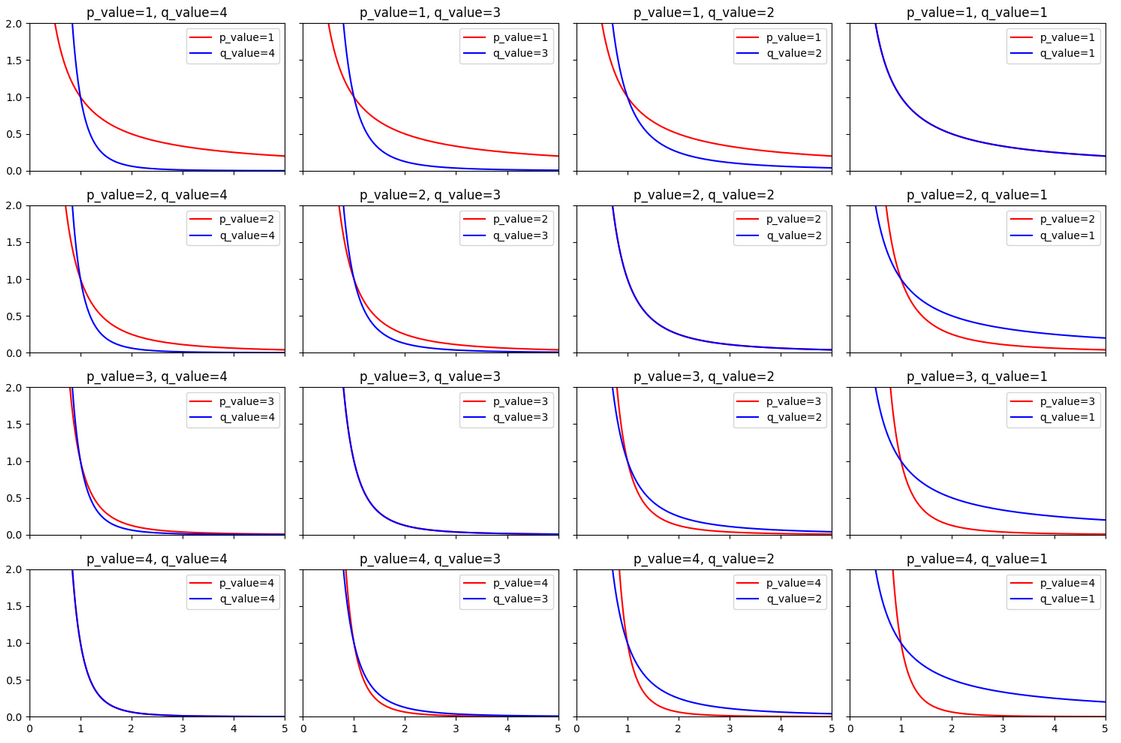
\includegraphics[width=1.3\textwidth]{graficas.png}
  \caption{Graphics in which both functions' behavior is shown}
  \label{fig:etiqueta}
\end{figure}

\end{document}